\documentclass{article}
\synctex=1
\usepackage[utf8]{inputenc}
%\usepackage{babel}
\usepackage{amsmath}
\usepackage{amssymb}
\usepackage{hyperref}
\usepackage{graphicx}
\usepackage{tikz}
\usepackage{pgf}
\usepackage{xcolor}
\usepackage[a4paper]{geometry}
\usepackage{csquotes}
\usepackage{listings}
\definecolor{light-gray}{gray}{0.95}
\definecolor{dark-blue}{rgb}{0, 0, 0.5}
\definecolor{dark-red}{rgb}{0.5, 0, 0}
\definecolor{dark-green}{rgb}{0, 0.5, 0}
\lstset{language=Python, backgroundcolor = \color{light-gray}}
\lstset{
language=Python, 
backgroundcolor = \color{light-gray},
basicstyle=\small\sffamily,
stringstyle=\color{orange},
breaklines=true,
keywordstyle=\bfseries\color{dark-blue}\textit, % Schlüsselwörter fett und schwarz drucken
commentstyle=\color{dark-green}, % Kommentare blau drucken
%stringstyle=\ttfamily, % Strings im Code Schreibmaschinenähnlich - setzt sich etwas vom Code ab
showstringspaces=false} % Strings im Code ohne Kenntlichmachung von Leerzeichen - finde ich angebracht und empfehlenswert
\newtheorem{defi}{Definition}[section]

% Kommentare beginnen mit dem Zeichen "%"

% Einstellung die verhindert, dass unschöne Rahmen um Links gezogen werden
\hypersetup{
    colorlinks = true, % false bedeutet Rahmen (nicht schön)
    linkcolor={red!20!black},
    citecolor={blue!50!black},
    urlcolor={blue!80!black},
}


% Abkürzungen einführen (alphabetische Sortierung empfehlenswert):

\newcommand{\ad}{\mathrm{ad}}
% renew weil \d schon belegt ist
\renewcommand{\d}{\mathrm{d}} % aufrechtes d (für Differentialformen)
\newcommand{\NV}{{\cal N}\,}
\newcommand{\rang}{\mathrm{rang}}
\newcommand{\im}{\mathrm{im}}
\newcommand{\spann}{\mathrm{span}}
\newcommand{\R}{\mathbb{R}} % doppeltes R
\newcommand{\py}{\emph{Python}\,}
\newcommand{\scipy}{\emph{SciPy}\,}
\newcommand{\mpl}{\emph{Matplotlib}\,}
\title{Control Theory Tutorial - Car-Like Mobile Robot}
%\institution{Institute of Control Theory - Technical University Dresden, Germany}
\date{}
\author{}
% Hier beginnt das eigentliche Dokument
\begin{document}
\maketitle
\section{Introduction}
The goal of this tutorial is to teach the usage of the programming language \py as a tool for developing and simulating control systems.
\section{Model of a car-like mobile robot}
\begin{figure}[ht]
	\centering
	\def\svgwidth{0.7\textwidth}
	\input{img/car-like_mobile_robot.pdf_tex}
	\caption{Car-like mobile robot}
	\label{fig:car}
\end{figure}
Given is a nonlinear kinematic model of a car-like mobile robot, with the following system variables: position $(y_1, y_2)$ and orientation $\theta$ in the plane, the steering angle $\phi$ and the robots lateral velocity $v=\left| \vec{v} \right| $. 
\begin{subequations}\label{eq:syseq}
\begin{align}
\dot{y_1}&=v \cos (\theta) \\
\dot{y_2}&=v \sin (\theta) \\
\tan(\phi) &= \frac{l\dot{\theta}}{v}
\end{align}
\end{subequations}
To simulate this system of 1st order ordinary differential equations (ODEs), we define a state vector $\mathbf{x}=(x_1,x_2,x_3)^\mathrm{T}$ and a control vector $\mathbf{u}=(u_1,u_2)^\mathrm{T}$:
\begin{align*}
x_1 &= y_1 & u_1 = v\\
x_2 &= y_2 & u_2 = \phi \\
x_3 &= \theta 
\end{align*}
Now we can express \eqref{eq:syseq} in a general form $\dot{\mathbf{x}}=f(\mathbf{x},\mathbf{u})$:
\label{eq:ss_system}
\begin{align}
\underbrace{\begin{pmatrix} \dot{x}_1 \\ \dot{x}_2 \\ \dot{x}_3 \end{pmatrix}}_{\dot{\mathbf{x}}} = \underbrace{\begin{pmatrix}  u_1 \cos(x_3) \\ u_1 \sin(x_3) \\ \frac{1}{l}u_1 \tan(u_2) \end{pmatrix}}_{f(\mathbf{x},\mathbf{u})}
\end{align}
\section{Storing parameters}
We store the parameters of our system in a class \emph{Parameters()}.
\begin{lstlisting}
class Parameters(object):
    pass
\end{lstlisting}
We therefore create an entity of \emph{Parameters()} and assign attributes.
\begin{lstlisting}
prmtrs = Parameters() # entity of class Parameters
prmtrs.l = 0.3 # define car length
prmtrs.w = prmtrs.l*0.3 # define car width
\end{lstlisting}
\section{Simulation with SciPy's integrate package}
\label{sec:simulation}
To simulate \eqref{eq:ss_system} we need to implement the ODE system as a function in \py.
\begin{lstlisting}
def ode(x, t, prmtrs):
    """Function of the robots kinematics

    Args:
        x: state
        t: time
        prmtrs(object): parameter container class

    Returns:
        dxdt: state derivative
    """
    x1, x2, x3 = x # state vector
    u1, u2 = control(x, t) # control vector
    # dxdt = f(x, u)
    dxdt = np.array([u1 * cos(x3),
                     u1 * sin(x3),
                     1 / prmtrs.l * u1 * tan(u2)])

    # return state derivative
    return dxdt
\end{lstlisting}
In order to use $\cos(\cdot), \sin(\cdot)$ and $\tan(\cdot)$ we need to import these functions at the beginning of our code from the \emph{numpy} library.
\begin{lstlisting}
import numpy as np 
from numpy import cos, sin, tan
\end{lstlisting}
The control law is also implemented as function.
\begin{lstlisting}
def control(x, t):
    """Function of the control law

    Args:
        x: state vector
        t: time

    Returns:
        u: control vector

    """
    u = [1, 0.25] # v, phi
    
    return u
\end{lstlisting}
As a first simple heuristic, we set $(u_1, u_2)$ equal to constant values. Later we can implement an arbitrary function, for expample a feedback law $\mathbf{u}=k(\mathbf{x})$.

\subsection{Solution of the initial value problem (IVP) using \scipy}
To simulate \eqref{eq:ss_system} we need to solve an IVP. In \py we can use the library \scipy and its sub-package \emph{integrate}, which delivers different solvers for IVPs.
\begin{lstlisting}
from scipy.integrate import odeint
\end{lstlisting}
We then define the simulation time and the initial state value.
\begin{lstlisting}
t0 = 0 # start 
tend = 10 # end
dt = 0.01 # stepsize (not of the solver, just evaluation points)
tt = np.arange(t0, tend, dt) # simulation interval

x0 = [0, 0, 0] # initial state value
\end{lstlisting}
Now we can parse these parameters and our ODE function to the solver.
\begin{lstlisting}
x_traj = odeint(ode, x0, tt, args=(prmtrs, )) # solution of the IVP
\end{lstlisting}
The output is an array of size length(tt)$\times$lenght($\mathbf{x}$).
\section{Plotting using \mpl}
\label{sec:plot}
For plotting the output of our simulation, we use the library \mpl and its sub-package \emph{pyplot}, which delivers a user experience similar to \emph{MATLAB}.
\begin{lstlisting}
import matplotlib.pyplot as plt
\end{lstlisting}
We encase our plotting instructions in a function. This way, we can define parameters of our plot, which we would like to change easily, for example figure width, or if the figure should be saved on the hard drive.
\begin{lstlisting}
def plot_data(fig_width, fig_height, save=False):
    """Plotting function of simulated state and actions

    Args:
        fig_width: figure width in cm
        fig_height: figure height in cm
        save (bool) : save figure (default: False)

    Returns: None

    """
    # creating a figure with 2 subplots, that share the x-axis
    fig1, (ax1, ax2) = plt.subplots(2, sharex=True)

    # set figure size to desired values
    fig1.set_size_inches(fig_width / 2.54, fig_height / 2.54)

    # plot y_1 in subplot 1
    ax1.plot(tt, x_traj[:, 0], label='$y_1(t)$', lw=1, color='r')

    # plot y_2 in subplot 1
    ax1.plot(tt, x_traj[:, 1], label='$y_2(t)$', lw=1, color='b')

    # plot theta in subplot 2
    ax2.plot(tt, x_traj[:, 2], label=r'$\theta(t)$', lw=1, color='g')

    ax1.grid(True)
    ax2.grid(True)
    # set the labels on the x and y axis in subplot 1
    ax1.set_ylabel(r'm')
    ax1.set_xlabel(r't in s')
    ax2.set_ylabel(r'rad')
    ax2.set_xlabel(r't in s')

    # put a legend in the plot
    ax1.legend()
    ax2.legend()

    #automatically adjusts subplot to fit in figure window
    plt.tight_layout()

    # save the figure in the working directory
    if save:
        plt.savefig('state_trajectory.pdf')  # save output as pdf
        plt.savefig('state_trajectory.pgf')  # for easy export to LaTex
    return None
\end{lstlisting}
Finally, we have to execute
\begin{lstlisting}
plt.show()
\end{lstlisting}
to display the results. If your not satisfied with the result, you can change other properties of the plot, like linewidth or -color and many others easily. Just look up the documentation of \mpl : \url{https://matplotlib.org/index.html}
\begin{figure}[h]
\label{fig:state_traj}
   \centering      
   %% Creator: Matplotlib, PGF backend
%%
%% To include the figure in your LaTeX document, write
%%   \input{<filename>.pgf}
%%
%% Make sure the required packages are loaded in your preamble
%%   \usepackage{pgf}
%%
%% Figures using additional raster images can only be included by \input if
%% they are in the same directory as the main LaTeX file. For loading figures
%% from other directories you can use the `import` package
%%   \usepackage{import}
%% and then include the figures with
%%   \import{<path to file>}{<filename>.pgf}
%%
%% Matplotlib used the following preamble
%%   \usepackage{fontspec}
%%   \setmainfont{Times New Roman}
%%   \setsansfont{Lucida Grande}
%%   \setmonofont{Andale Mono}
%%
\begingroup%
\makeatletter%
\begin{pgfpicture}%
\pgfpathrectangle{\pgfpointorigin}{\pgfqpoint{4.724409in}{3.149606in}}%
\pgfusepath{use as bounding box, clip}%
\begin{pgfscope}%
\pgfsetbuttcap%
\pgfsetmiterjoin%
\definecolor{currentfill}{rgb}{1.000000,1.000000,1.000000}%
\pgfsetfillcolor{currentfill}%
\pgfsetlinewidth{0.000000pt}%
\definecolor{currentstroke}{rgb}{1.000000,1.000000,1.000000}%
\pgfsetstrokecolor{currentstroke}%
\pgfsetdash{}{0pt}%
\pgfpathmoveto{\pgfqpoint{0.000000in}{0.000000in}}%
\pgfpathlineto{\pgfqpoint{4.724409in}{0.000000in}}%
\pgfpathlineto{\pgfqpoint{4.724409in}{3.149606in}}%
\pgfpathlineto{\pgfqpoint{0.000000in}{3.149606in}}%
\pgfpathclose%
\pgfusepath{fill}%
\end{pgfscope}%
\begin{pgfscope}%
\pgfsetbuttcap%
\pgfsetmiterjoin%
\definecolor{currentfill}{rgb}{1.000000,1.000000,1.000000}%
\pgfsetfillcolor{currentfill}%
\pgfsetlinewidth{0.000000pt}%
\definecolor{currentstroke}{rgb}{0.000000,0.000000,0.000000}%
\pgfsetstrokecolor{currentstroke}%
\pgfsetstrokeopacity{0.000000}%
\pgfsetdash{}{0pt}%
\pgfpathmoveto{\pgfqpoint{0.530278in}{1.963970in}}%
\pgfpathlineto{\pgfqpoint{4.539409in}{1.963970in}}%
\pgfpathlineto{\pgfqpoint{4.539409in}{2.964606in}}%
\pgfpathlineto{\pgfqpoint{0.530278in}{2.964606in}}%
\pgfpathclose%
\pgfusepath{fill}%
\end{pgfscope}%
\begin{pgfscope}%
\pgfpathrectangle{\pgfqpoint{0.530278in}{1.963970in}}{\pgfqpoint{4.009132in}{1.000636in}} %
\pgfusepath{clip}%
\pgfsetrectcap%
\pgfsetroundjoin%
\pgfsetlinewidth{0.803000pt}%
\definecolor{currentstroke}{rgb}{0.690196,0.690196,0.690196}%
\pgfsetstrokecolor{currentstroke}%
\pgfsetdash{}{0pt}%
\pgfpathmoveto{\pgfqpoint{0.712511in}{1.963970in}}%
\pgfpathlineto{\pgfqpoint{0.712511in}{2.964606in}}%
\pgfusepath{stroke}%
\end{pgfscope}%
\begin{pgfscope}%
\pgfsetbuttcap%
\pgfsetroundjoin%
\definecolor{currentfill}{rgb}{0.000000,0.000000,0.000000}%
\pgfsetfillcolor{currentfill}%
\pgfsetlinewidth{0.803000pt}%
\definecolor{currentstroke}{rgb}{0.000000,0.000000,0.000000}%
\pgfsetstrokecolor{currentstroke}%
\pgfsetdash{}{0pt}%
\pgfsys@defobject{currentmarker}{\pgfqpoint{0.000000in}{-0.048611in}}{\pgfqpoint{0.000000in}{0.000000in}}{%
\pgfpathmoveto{\pgfqpoint{0.000000in}{0.000000in}}%
\pgfpathlineto{\pgfqpoint{0.000000in}{-0.048611in}}%
\pgfusepath{stroke,fill}%
}%
\begin{pgfscope}%
\pgfsys@transformshift{0.712511in}{1.963970in}%
\pgfsys@useobject{currentmarker}{}%
\end{pgfscope}%
\end{pgfscope}%
\begin{pgfscope}%
\pgfpathrectangle{\pgfqpoint{0.530278in}{1.963970in}}{\pgfqpoint{4.009132in}{1.000636in}} %
\pgfusepath{clip}%
\pgfsetrectcap%
\pgfsetroundjoin%
\pgfsetlinewidth{0.803000pt}%
\definecolor{currentstroke}{rgb}{0.690196,0.690196,0.690196}%
\pgfsetstrokecolor{currentstroke}%
\pgfsetdash{}{0pt}%
\pgfpathmoveto{\pgfqpoint{1.444372in}{1.963970in}}%
\pgfpathlineto{\pgfqpoint{1.444372in}{2.964606in}}%
\pgfusepath{stroke}%
\end{pgfscope}%
\begin{pgfscope}%
\pgfsetbuttcap%
\pgfsetroundjoin%
\definecolor{currentfill}{rgb}{0.000000,0.000000,0.000000}%
\pgfsetfillcolor{currentfill}%
\pgfsetlinewidth{0.803000pt}%
\definecolor{currentstroke}{rgb}{0.000000,0.000000,0.000000}%
\pgfsetstrokecolor{currentstroke}%
\pgfsetdash{}{0pt}%
\pgfsys@defobject{currentmarker}{\pgfqpoint{0.000000in}{-0.048611in}}{\pgfqpoint{0.000000in}{0.000000in}}{%
\pgfpathmoveto{\pgfqpoint{0.000000in}{0.000000in}}%
\pgfpathlineto{\pgfqpoint{0.000000in}{-0.048611in}}%
\pgfusepath{stroke,fill}%
}%
\begin{pgfscope}%
\pgfsys@transformshift{1.444372in}{1.963970in}%
\pgfsys@useobject{currentmarker}{}%
\end{pgfscope}%
\end{pgfscope}%
\begin{pgfscope}%
\pgfpathrectangle{\pgfqpoint{0.530278in}{1.963970in}}{\pgfqpoint{4.009132in}{1.000636in}} %
\pgfusepath{clip}%
\pgfsetrectcap%
\pgfsetroundjoin%
\pgfsetlinewidth{0.803000pt}%
\definecolor{currentstroke}{rgb}{0.690196,0.690196,0.690196}%
\pgfsetstrokecolor{currentstroke}%
\pgfsetdash{}{0pt}%
\pgfpathmoveto{\pgfqpoint{2.176232in}{1.963970in}}%
\pgfpathlineto{\pgfqpoint{2.176232in}{2.964606in}}%
\pgfusepath{stroke}%
\end{pgfscope}%
\begin{pgfscope}%
\pgfsetbuttcap%
\pgfsetroundjoin%
\definecolor{currentfill}{rgb}{0.000000,0.000000,0.000000}%
\pgfsetfillcolor{currentfill}%
\pgfsetlinewidth{0.803000pt}%
\definecolor{currentstroke}{rgb}{0.000000,0.000000,0.000000}%
\pgfsetstrokecolor{currentstroke}%
\pgfsetdash{}{0pt}%
\pgfsys@defobject{currentmarker}{\pgfqpoint{0.000000in}{-0.048611in}}{\pgfqpoint{0.000000in}{0.000000in}}{%
\pgfpathmoveto{\pgfqpoint{0.000000in}{0.000000in}}%
\pgfpathlineto{\pgfqpoint{0.000000in}{-0.048611in}}%
\pgfusepath{stroke,fill}%
}%
\begin{pgfscope}%
\pgfsys@transformshift{2.176232in}{1.963970in}%
\pgfsys@useobject{currentmarker}{}%
\end{pgfscope}%
\end{pgfscope}%
\begin{pgfscope}%
\pgfpathrectangle{\pgfqpoint{0.530278in}{1.963970in}}{\pgfqpoint{4.009132in}{1.000636in}} %
\pgfusepath{clip}%
\pgfsetrectcap%
\pgfsetroundjoin%
\pgfsetlinewidth{0.803000pt}%
\definecolor{currentstroke}{rgb}{0.690196,0.690196,0.690196}%
\pgfsetstrokecolor{currentstroke}%
\pgfsetdash{}{0pt}%
\pgfpathmoveto{\pgfqpoint{2.908092in}{1.963970in}}%
\pgfpathlineto{\pgfqpoint{2.908092in}{2.964606in}}%
\pgfusepath{stroke}%
\end{pgfscope}%
\begin{pgfscope}%
\pgfsetbuttcap%
\pgfsetroundjoin%
\definecolor{currentfill}{rgb}{0.000000,0.000000,0.000000}%
\pgfsetfillcolor{currentfill}%
\pgfsetlinewidth{0.803000pt}%
\definecolor{currentstroke}{rgb}{0.000000,0.000000,0.000000}%
\pgfsetstrokecolor{currentstroke}%
\pgfsetdash{}{0pt}%
\pgfsys@defobject{currentmarker}{\pgfqpoint{0.000000in}{-0.048611in}}{\pgfqpoint{0.000000in}{0.000000in}}{%
\pgfpathmoveto{\pgfqpoint{0.000000in}{0.000000in}}%
\pgfpathlineto{\pgfqpoint{0.000000in}{-0.048611in}}%
\pgfusepath{stroke,fill}%
}%
\begin{pgfscope}%
\pgfsys@transformshift{2.908092in}{1.963970in}%
\pgfsys@useobject{currentmarker}{}%
\end{pgfscope}%
\end{pgfscope}%
\begin{pgfscope}%
\pgfpathrectangle{\pgfqpoint{0.530278in}{1.963970in}}{\pgfqpoint{4.009132in}{1.000636in}} %
\pgfusepath{clip}%
\pgfsetrectcap%
\pgfsetroundjoin%
\pgfsetlinewidth{0.803000pt}%
\definecolor{currentstroke}{rgb}{0.690196,0.690196,0.690196}%
\pgfsetstrokecolor{currentstroke}%
\pgfsetdash{}{0pt}%
\pgfpathmoveto{\pgfqpoint{3.639953in}{1.963970in}}%
\pgfpathlineto{\pgfqpoint{3.639953in}{2.964606in}}%
\pgfusepath{stroke}%
\end{pgfscope}%
\begin{pgfscope}%
\pgfsetbuttcap%
\pgfsetroundjoin%
\definecolor{currentfill}{rgb}{0.000000,0.000000,0.000000}%
\pgfsetfillcolor{currentfill}%
\pgfsetlinewidth{0.803000pt}%
\definecolor{currentstroke}{rgb}{0.000000,0.000000,0.000000}%
\pgfsetstrokecolor{currentstroke}%
\pgfsetdash{}{0pt}%
\pgfsys@defobject{currentmarker}{\pgfqpoint{0.000000in}{-0.048611in}}{\pgfqpoint{0.000000in}{0.000000in}}{%
\pgfpathmoveto{\pgfqpoint{0.000000in}{0.000000in}}%
\pgfpathlineto{\pgfqpoint{0.000000in}{-0.048611in}}%
\pgfusepath{stroke,fill}%
}%
\begin{pgfscope}%
\pgfsys@transformshift{3.639953in}{1.963970in}%
\pgfsys@useobject{currentmarker}{}%
\end{pgfscope}%
\end{pgfscope}%
\begin{pgfscope}%
\pgfpathrectangle{\pgfqpoint{0.530278in}{1.963970in}}{\pgfqpoint{4.009132in}{1.000636in}} %
\pgfusepath{clip}%
\pgfsetrectcap%
\pgfsetroundjoin%
\pgfsetlinewidth{0.803000pt}%
\definecolor{currentstroke}{rgb}{0.690196,0.690196,0.690196}%
\pgfsetstrokecolor{currentstroke}%
\pgfsetdash{}{0pt}%
\pgfpathmoveto{\pgfqpoint{4.371813in}{1.963970in}}%
\pgfpathlineto{\pgfqpoint{4.371813in}{2.964606in}}%
\pgfusepath{stroke}%
\end{pgfscope}%
\begin{pgfscope}%
\pgfsetbuttcap%
\pgfsetroundjoin%
\definecolor{currentfill}{rgb}{0.000000,0.000000,0.000000}%
\pgfsetfillcolor{currentfill}%
\pgfsetlinewidth{0.803000pt}%
\definecolor{currentstroke}{rgb}{0.000000,0.000000,0.000000}%
\pgfsetstrokecolor{currentstroke}%
\pgfsetdash{}{0pt}%
\pgfsys@defobject{currentmarker}{\pgfqpoint{0.000000in}{-0.048611in}}{\pgfqpoint{0.000000in}{0.000000in}}{%
\pgfpathmoveto{\pgfqpoint{0.000000in}{0.000000in}}%
\pgfpathlineto{\pgfqpoint{0.000000in}{-0.048611in}}%
\pgfusepath{stroke,fill}%
}%
\begin{pgfscope}%
\pgfsys@transformshift{4.371813in}{1.963970in}%
\pgfsys@useobject{currentmarker}{}%
\end{pgfscope}%
\end{pgfscope}%
\begin{pgfscope}%
\pgftext[x=2.534844in,y=1.908414in,,top]{\sffamily\fontsize{10.000000}{12.000000}\selectfont t in s}%
\end{pgfscope}%
\begin{pgfscope}%
\pgfpathrectangle{\pgfqpoint{0.530278in}{1.963970in}}{\pgfqpoint{4.009132in}{1.000636in}} %
\pgfusepath{clip}%
\pgfsetrectcap%
\pgfsetroundjoin%
\pgfsetlinewidth{0.803000pt}%
\definecolor{currentstroke}{rgb}{0.690196,0.690196,0.690196}%
\pgfsetstrokecolor{currentstroke}%
\pgfsetdash{}{0pt}%
\pgfpathmoveto{\pgfqpoint{0.530278in}{2.312661in}}%
\pgfpathlineto{\pgfqpoint{4.539409in}{2.312661in}}%
\pgfusepath{stroke}%
\end{pgfscope}%
\begin{pgfscope}%
\pgfsetbuttcap%
\pgfsetroundjoin%
\definecolor{currentfill}{rgb}{0.000000,0.000000,0.000000}%
\pgfsetfillcolor{currentfill}%
\pgfsetlinewidth{0.803000pt}%
\definecolor{currentstroke}{rgb}{0.000000,0.000000,0.000000}%
\pgfsetstrokecolor{currentstroke}%
\pgfsetdash{}{0pt}%
\pgfsys@defobject{currentmarker}{\pgfqpoint{-0.048611in}{0.000000in}}{\pgfqpoint{0.000000in}{0.000000in}}{%
\pgfpathmoveto{\pgfqpoint{0.000000in}{0.000000in}}%
\pgfpathlineto{\pgfqpoint{-0.048611in}{0.000000in}}%
\pgfusepath{stroke,fill}%
}%
\begin{pgfscope}%
\pgfsys@transformshift{0.530278in}{2.312661in}%
\pgfsys@useobject{currentmarker}{}%
\end{pgfscope}%
\end{pgfscope}%
\begin{pgfscope}%
\pgftext[x=0.345233in,y=2.259119in,left,base]{\sffamily\fontsize{10.000000}{12.000000}\selectfont 0}%
\end{pgfscope}%
\begin{pgfscope}%
\pgfpathrectangle{\pgfqpoint{0.530278in}{1.963970in}}{\pgfqpoint{4.009132in}{1.000636in}} %
\pgfusepath{clip}%
\pgfsetrectcap%
\pgfsetroundjoin%
\pgfsetlinewidth{0.803000pt}%
\definecolor{currentstroke}{rgb}{0.690196,0.690196,0.690196}%
\pgfsetstrokecolor{currentstroke}%
\pgfsetdash{}{0pt}%
\pgfpathmoveto{\pgfqpoint{0.530278in}{2.828856in}}%
\pgfpathlineto{\pgfqpoint{4.539409in}{2.828856in}}%
\pgfusepath{stroke}%
\end{pgfscope}%
\begin{pgfscope}%
\pgfsetbuttcap%
\pgfsetroundjoin%
\definecolor{currentfill}{rgb}{0.000000,0.000000,0.000000}%
\pgfsetfillcolor{currentfill}%
\pgfsetlinewidth{0.803000pt}%
\definecolor{currentstroke}{rgb}{0.000000,0.000000,0.000000}%
\pgfsetstrokecolor{currentstroke}%
\pgfsetdash{}{0pt}%
\pgfsys@defobject{currentmarker}{\pgfqpoint{-0.048611in}{0.000000in}}{\pgfqpoint{0.000000in}{0.000000in}}{%
\pgfpathmoveto{\pgfqpoint{0.000000in}{0.000000in}}%
\pgfpathlineto{\pgfqpoint{-0.048611in}{0.000000in}}%
\pgfusepath{stroke,fill}%
}%
\begin{pgfscope}%
\pgfsys@transformshift{0.530278in}{2.828856in}%
\pgfsys@useobject{currentmarker}{}%
\end{pgfscope}%
\end{pgfscope}%
\begin{pgfscope}%
\pgftext[x=0.345233in,y=2.775315in,left,base]{\sffamily\fontsize{10.000000}{12.000000}\selectfont 2}%
\end{pgfscope}%
\begin{pgfscope}%
\pgftext[x=0.289677in,y=2.464288in,,bottom,rotate=90.000000]{\sffamily\fontsize{10.000000}{12.000000}\selectfont m}%
\end{pgfscope}%
\begin{pgfscope}%
\pgfpathrectangle{\pgfqpoint{0.530278in}{1.963970in}}{\pgfqpoint{4.009132in}{1.000636in}} %
\pgfusepath{clip}%
\pgfsetrectcap%
\pgfsetroundjoin%
\pgfsetlinewidth{1.003750pt}%
\definecolor{currentstroke}{rgb}{1.000000,0.000000,0.000000}%
\pgfsetstrokecolor{currentstroke}%
\pgfsetdash{}{0pt}%
\pgfpathmoveto{\pgfqpoint{0.712511in}{2.312661in}}%
\pgfpathlineto{\pgfqpoint{0.829609in}{2.394235in}}%
\pgfpathlineto{\pgfqpoint{0.902795in}{2.442533in}}%
\pgfpathlineto{\pgfqpoint{0.961344in}{2.478532in}}%
\pgfpathlineto{\pgfqpoint{1.019892in}{2.511459in}}%
\pgfpathlineto{\pgfqpoint{1.063804in}{2.533770in}}%
\pgfpathlineto{\pgfqpoint{1.107716in}{2.553776in}}%
\pgfpathlineto{\pgfqpoint{1.151627in}{2.571269in}}%
\pgfpathlineto{\pgfqpoint{1.195539in}{2.586067in}}%
\pgfpathlineto{\pgfqpoint{1.239451in}{2.598014in}}%
\pgfpathlineto{\pgfqpoint{1.283362in}{2.606988in}}%
\pgfpathlineto{\pgfqpoint{1.327274in}{2.612894in}}%
\pgfpathlineto{\pgfqpoint{1.371185in}{2.615671in}}%
\pgfpathlineto{\pgfqpoint{1.415097in}{2.615289in}}%
\pgfpathlineto{\pgfqpoint{1.459009in}{2.611754in}}%
\pgfpathlineto{\pgfqpoint{1.502920in}{2.605101in}}%
\pgfpathlineto{\pgfqpoint{1.546832in}{2.595399in}}%
\pgfpathlineto{\pgfqpoint{1.590744in}{2.582751in}}%
\pgfpathlineto{\pgfqpoint{1.634655in}{2.567288in}}%
\pgfpathlineto{\pgfqpoint{1.678567in}{2.549171in}}%
\pgfpathlineto{\pgfqpoint{1.722478in}{2.528588in}}%
\pgfpathlineto{\pgfqpoint{1.766390in}{2.505755in}}%
\pgfpathlineto{\pgfqpoint{1.824939in}{2.472225in}}%
\pgfpathlineto{\pgfqpoint{1.883488in}{2.435740in}}%
\pgfpathlineto{\pgfqpoint{1.956674in}{2.387012in}}%
\pgfpathlineto{\pgfqpoint{2.059134in}{2.315511in}}%
\pgfpathlineto{\pgfqpoint{2.190869in}{2.223914in}}%
\pgfpathlineto{\pgfqpoint{2.264055in}{2.176075in}}%
\pgfpathlineto{\pgfqpoint{2.322604in}{2.140584in}}%
\pgfpathlineto{\pgfqpoint{2.366516in}{2.116024in}}%
\pgfpathlineto{\pgfqpoint{2.410427in}{2.093512in}}%
\pgfpathlineto{\pgfqpoint{2.454339in}{2.073285in}}%
\pgfpathlineto{\pgfqpoint{2.498251in}{2.055552in}}%
\pgfpathlineto{\pgfqpoint{2.542162in}{2.040500in}}%
\pgfpathlineto{\pgfqpoint{2.586074in}{2.028284in}}%
\pgfpathlineto{\pgfqpoint{2.629985in}{2.019032in}}%
\pgfpathlineto{\pgfqpoint{2.673897in}{2.012841in}}%
\pgfpathlineto{\pgfqpoint{2.717809in}{2.009775in}}%
\pgfpathlineto{\pgfqpoint{2.761720in}{2.009865in}}%
\pgfpathlineto{\pgfqpoint{2.805632in}{2.013112in}}%
\pgfpathlineto{\pgfqpoint{2.849544in}{2.019480in}}%
\pgfpathlineto{\pgfqpoint{2.893455in}{2.028905in}}%
\pgfpathlineto{\pgfqpoint{2.937367in}{2.041287in}}%
\pgfpathlineto{\pgfqpoint{2.981279in}{2.056497in}}%
\pgfpathlineto{\pgfqpoint{3.025190in}{2.074378in}}%
\pgfpathlineto{\pgfqpoint{3.069102in}{2.094742in}}%
\pgfpathlineto{\pgfqpoint{3.113013in}{2.117377in}}%
\pgfpathlineto{\pgfqpoint{3.171562in}{2.150680in}}%
\pgfpathlineto{\pgfqpoint{3.230111in}{2.186982in}}%
\pgfpathlineto{\pgfqpoint{3.303297in}{2.235550in}}%
\pgfpathlineto{\pgfqpoint{3.405758in}{2.306961in}}%
\pgfpathlineto{\pgfqpoint{3.537492in}{2.398679in}}%
\pgfpathlineto{\pgfqpoint{3.610679in}{2.446696in}}%
\pgfpathlineto{\pgfqpoint{3.669227in}{2.482383in}}%
\pgfpathlineto{\pgfqpoint{3.727776in}{2.514927in}}%
\pgfpathlineto{\pgfqpoint{3.771688in}{2.536908in}}%
\pgfpathlineto{\pgfqpoint{3.815599in}{2.556552in}}%
\pgfpathlineto{\pgfqpoint{3.859511in}{2.573653in}}%
\pgfpathlineto{\pgfqpoint{3.903423in}{2.588035in}}%
\pgfpathlineto{\pgfqpoint{3.947334in}{2.599546in}}%
\pgfpathlineto{\pgfqpoint{3.991246in}{2.608067in}}%
\pgfpathlineto{\pgfqpoint{4.035158in}{2.613509in}}%
\pgfpathlineto{\pgfqpoint{4.079069in}{2.615815in}}%
\pgfpathlineto{\pgfqpoint{4.122981in}{2.614961in}}%
\pgfpathlineto{\pgfqpoint{4.166892in}{2.610957in}}%
\pgfpathlineto{\pgfqpoint{4.210804in}{2.603844in}}%
\pgfpathlineto{\pgfqpoint{4.254716in}{2.593695in}}%
\pgfpathlineto{\pgfqpoint{4.298627in}{2.580618in}}%
\pgfpathlineto{\pgfqpoint{4.342539in}{2.564747in}}%
\pgfpathlineto{\pgfqpoint{4.357176in}{2.558864in}}%
\pgfpathlineto{\pgfqpoint{4.357176in}{2.558864in}}%
\pgfusepath{stroke}%
\end{pgfscope}%
\begin{pgfscope}%
\pgfpathrectangle{\pgfqpoint{0.530278in}{1.963970in}}{\pgfqpoint{4.009132in}{1.000636in}} %
\pgfusepath{clip}%
\pgfsetrectcap%
\pgfsetroundjoin%
\pgfsetlinewidth{1.003750pt}%
\definecolor{currentstroke}{rgb}{0.000000,0.000000,1.000000}%
\pgfsetstrokecolor{currentstroke}%
\pgfsetdash{}{0pt}%
\pgfpathmoveto{\pgfqpoint{0.712511in}{2.312661in}}%
\pgfpathlineto{\pgfqpoint{0.756423in}{2.314241in}}%
\pgfpathlineto{\pgfqpoint{0.800334in}{2.318966in}}%
\pgfpathlineto{\pgfqpoint{0.844246in}{2.326785in}}%
\pgfpathlineto{\pgfqpoint{0.888158in}{2.337618in}}%
\pgfpathlineto{\pgfqpoint{0.932069in}{2.351351in}}%
\pgfpathlineto{\pgfqpoint{0.975981in}{2.367841in}}%
\pgfpathlineto{\pgfqpoint{1.019892in}{2.386917in}}%
\pgfpathlineto{\pgfqpoint{1.063804in}{2.408380in}}%
\pgfpathlineto{\pgfqpoint{1.107716in}{2.432006in}}%
\pgfpathlineto{\pgfqpoint{1.166265in}{2.466442in}}%
\pgfpathlineto{\pgfqpoint{1.224813in}{2.503647in}}%
\pgfpathlineto{\pgfqpoint{1.297999in}{2.552990in}}%
\pgfpathlineto{\pgfqpoint{1.444372in}{2.655654in}}%
\pgfpathlineto{\pgfqpoint{1.532195in}{2.715810in}}%
\pgfpathlineto{\pgfqpoint{1.590744in}{2.753755in}}%
\pgfpathlineto{\pgfqpoint{1.649292in}{2.789146in}}%
\pgfpathlineto{\pgfqpoint{1.693204in}{2.813618in}}%
\pgfpathlineto{\pgfqpoint{1.737116in}{2.836030in}}%
\pgfpathlineto{\pgfqpoint{1.781027in}{2.856147in}}%
\pgfpathlineto{\pgfqpoint{1.824939in}{2.873760in}}%
\pgfpathlineto{\pgfqpoint{1.868851in}{2.888685in}}%
\pgfpathlineto{\pgfqpoint{1.912762in}{2.900767in}}%
\pgfpathlineto{\pgfqpoint{1.956674in}{2.909880in}}%
\pgfpathlineto{\pgfqpoint{2.000585in}{2.915929in}}%
\pgfpathlineto{\pgfqpoint{2.044497in}{2.918850in}}%
\pgfpathlineto{\pgfqpoint{2.088409in}{2.918614in}}%
\pgfpathlineto{\pgfqpoint{2.132320in}{2.915223in}}%
\pgfpathlineto{\pgfqpoint{2.176232in}{2.908712in}}%
\pgfpathlineto{\pgfqpoint{2.220144in}{2.899149in}}%
\pgfpathlineto{\pgfqpoint{2.264055in}{2.886634in}}%
\pgfpathlineto{\pgfqpoint{2.307967in}{2.871297in}}%
\pgfpathlineto{\pgfqpoint{2.351878in}{2.853298in}}%
\pgfpathlineto{\pgfqpoint{2.395790in}{2.832824in}}%
\pgfpathlineto{\pgfqpoint{2.439702in}{2.810090in}}%
\pgfpathlineto{\pgfqpoint{2.498251in}{2.776673in}}%
\pgfpathlineto{\pgfqpoint{2.556799in}{2.740279in}}%
\pgfpathlineto{\pgfqpoint{2.629985in}{2.691631in}}%
\pgfpathlineto{\pgfqpoint{2.732446in}{2.620173in}}%
\pgfpathlineto{\pgfqpoint{2.864181in}{2.528515in}}%
\pgfpathlineto{\pgfqpoint{2.937367in}{2.480587in}}%
\pgfpathlineto{\pgfqpoint{2.995916in}{2.444997in}}%
\pgfpathlineto{\pgfqpoint{3.039827in}{2.420348in}}%
\pgfpathlineto{\pgfqpoint{3.083739in}{2.397737in}}%
\pgfpathlineto{\pgfqpoint{3.127651in}{2.377400in}}%
\pgfpathlineto{\pgfqpoint{3.171562in}{2.359548in}}%
\pgfpathlineto{\pgfqpoint{3.215474in}{2.344369in}}%
\pgfpathlineto{\pgfqpoint{3.259385in}{2.332020in}}%
\pgfpathlineto{\pgfqpoint{3.303297in}{2.322629in}}%
\pgfpathlineto{\pgfqpoint{3.347209in}{2.316295in}}%
\pgfpathlineto{\pgfqpoint{3.391120in}{2.313084in}}%
\pgfpathlineto{\pgfqpoint{3.435032in}{2.313029in}}%
\pgfpathlineto{\pgfqpoint{3.478944in}{2.316131in}}%
\pgfpathlineto{\pgfqpoint{3.522855in}{2.322357in}}%
\pgfpathlineto{\pgfqpoint{3.566767in}{2.331643in}}%
\pgfpathlineto{\pgfqpoint{3.610679in}{2.343892in}}%
\pgfpathlineto{\pgfqpoint{3.654590in}{2.358975in}}%
\pgfpathlineto{\pgfqpoint{3.698502in}{2.376737in}}%
\pgfpathlineto{\pgfqpoint{3.742413in}{2.396991in}}%
\pgfpathlineto{\pgfqpoint{3.786325in}{2.419527in}}%
\pgfpathlineto{\pgfqpoint{3.830237in}{2.444110in}}%
\pgfpathlineto{\pgfqpoint{3.888785in}{2.479625in}}%
\pgfpathlineto{\pgfqpoint{3.947334in}{2.517663in}}%
\pgfpathlineto{\pgfqpoint{4.035158in}{2.577902in}}%
\pgfpathlineto{\pgfqpoint{4.225441in}{2.710411in}}%
\pgfpathlineto{\pgfqpoint{4.298627in}{2.757857in}}%
\pgfpathlineto{\pgfqpoint{4.357176in}{2.792921in}}%
\pgfpathlineto{\pgfqpoint{4.357176in}{2.792921in}}%
\pgfusepath{stroke}%
\end{pgfscope}%
\begin{pgfscope}%
\pgfsetrectcap%
\pgfsetmiterjoin%
\pgfsetlinewidth{0.803000pt}%
\definecolor{currentstroke}{rgb}{0.000000,0.000000,0.000000}%
\pgfsetstrokecolor{currentstroke}%
\pgfsetdash{}{0pt}%
\pgfpathmoveto{\pgfqpoint{0.530278in}{1.963970in}}%
\pgfpathlineto{\pgfqpoint{0.530278in}{2.964606in}}%
\pgfusepath{stroke}%
\end{pgfscope}%
\begin{pgfscope}%
\pgfsetrectcap%
\pgfsetmiterjoin%
\pgfsetlinewidth{0.803000pt}%
\definecolor{currentstroke}{rgb}{0.000000,0.000000,0.000000}%
\pgfsetstrokecolor{currentstroke}%
\pgfsetdash{}{0pt}%
\pgfpathmoveto{\pgfqpoint{4.539409in}{1.963970in}}%
\pgfpathlineto{\pgfqpoint{4.539409in}{2.964606in}}%
\pgfusepath{stroke}%
\end{pgfscope}%
\begin{pgfscope}%
\pgfsetrectcap%
\pgfsetmiterjoin%
\pgfsetlinewidth{0.803000pt}%
\definecolor{currentstroke}{rgb}{0.000000,0.000000,0.000000}%
\pgfsetstrokecolor{currentstroke}%
\pgfsetdash{}{0pt}%
\pgfpathmoveto{\pgfqpoint{0.530278in}{1.963970in}}%
\pgfpathlineto{\pgfqpoint{4.539409in}{1.963970in}}%
\pgfusepath{stroke}%
\end{pgfscope}%
\begin{pgfscope}%
\pgfsetrectcap%
\pgfsetmiterjoin%
\pgfsetlinewidth{0.803000pt}%
\definecolor{currentstroke}{rgb}{0.000000,0.000000,0.000000}%
\pgfsetstrokecolor{currentstroke}%
\pgfsetdash{}{0pt}%
\pgfpathmoveto{\pgfqpoint{0.530278in}{2.964606in}}%
\pgfpathlineto{\pgfqpoint{4.539409in}{2.964606in}}%
\pgfusepath{stroke}%
\end{pgfscope}%
\begin{pgfscope}%
\pgfsetbuttcap%
\pgfsetmiterjoin%
\definecolor{currentfill}{rgb}{1.000000,1.000000,1.000000}%
\pgfsetfillcolor{currentfill}%
\pgfsetfillopacity{0.800000}%
\pgfsetlinewidth{1.003750pt}%
\definecolor{currentstroke}{rgb}{0.800000,0.800000,0.800000}%
\pgfsetstrokecolor{currentstroke}%
\pgfsetstrokeopacity{0.800000}%
\pgfsetdash{}{0pt}%
\pgfpathmoveto{\pgfqpoint{3.709161in}{2.033414in}}%
\pgfpathlineto{\pgfqpoint{4.442187in}{2.033414in}}%
\pgfpathquadraticcurveto{\pgfqpoint{4.469965in}{2.033414in}}{\pgfqpoint{4.469965in}{2.061192in}}%
\pgfpathlineto{\pgfqpoint{4.469965in}{2.469802in}}%
\pgfpathquadraticcurveto{\pgfqpoint{4.469965in}{2.497580in}}{\pgfqpoint{4.442187in}{2.497580in}}%
\pgfpathlineto{\pgfqpoint{3.709161in}{2.497580in}}%
\pgfpathquadraticcurveto{\pgfqpoint{3.681384in}{2.497580in}}{\pgfqpoint{3.681384in}{2.469802in}}%
\pgfpathlineto{\pgfqpoint{3.681384in}{2.061192in}}%
\pgfpathquadraticcurveto{\pgfqpoint{3.681384in}{2.033414in}}{\pgfqpoint{3.709161in}{2.033414in}}%
\pgfpathclose%
\pgfusepath{stroke,fill}%
\end{pgfscope}%
\begin{pgfscope}%
\pgfsetrectcap%
\pgfsetroundjoin%
\pgfsetlinewidth{1.003750pt}%
\definecolor{currentstroke}{rgb}{1.000000,0.000000,0.000000}%
\pgfsetstrokecolor{currentstroke}%
\pgfsetdash{}{0pt}%
\pgfpathmoveto{\pgfqpoint{3.736939in}{2.383553in}}%
\pgfpathlineto{\pgfqpoint{4.014717in}{2.383553in}}%
\pgfusepath{stroke}%
\end{pgfscope}%
\begin{pgfscope}%
\pgftext[x=4.125828in,y=2.334941in,left,base]{\sffamily\fontsize{10.000000}{12.000000}\selectfont \(\displaystyle y_1(t)\)}%
\end{pgfscope}%
\begin{pgfscope}%
\pgfsetrectcap%
\pgfsetroundjoin%
\pgfsetlinewidth{1.003750pt}%
\definecolor{currentstroke}{rgb}{0.000000,0.000000,1.000000}%
\pgfsetstrokecolor{currentstroke}%
\pgfsetdash{}{0pt}%
\pgfpathmoveto{\pgfqpoint{3.736939in}{2.172303in}}%
\pgfpathlineto{\pgfqpoint{4.014717in}{2.172303in}}%
\pgfusepath{stroke}%
\end{pgfscope}%
\begin{pgfscope}%
\pgftext[x=4.125828in,y=2.123692in,left,base]{\sffamily\fontsize{10.000000}{12.000000}\selectfont \(\displaystyle y_2(t)\)}%
\end{pgfscope}%
\begin{pgfscope}%
\pgfsetbuttcap%
\pgfsetmiterjoin%
\definecolor{currentfill}{rgb}{1.000000,1.000000,1.000000}%
\pgfsetfillcolor{currentfill}%
\pgfsetlinewidth{0.000000pt}%
\definecolor{currentstroke}{rgb}{0.000000,0.000000,0.000000}%
\pgfsetstrokecolor{currentstroke}%
\pgfsetstrokeopacity{0.000000}%
\pgfsetdash{}{0pt}%
\pgfpathmoveto{\pgfqpoint{0.530278in}{0.582778in}}%
\pgfpathlineto{\pgfqpoint{4.539409in}{0.582778in}}%
\pgfpathlineto{\pgfqpoint{4.539409in}{1.583414in}}%
\pgfpathlineto{\pgfqpoint{0.530278in}{1.583414in}}%
\pgfpathclose%
\pgfusepath{fill}%
\end{pgfscope}%
\begin{pgfscope}%
\pgfpathrectangle{\pgfqpoint{0.530278in}{0.582778in}}{\pgfqpoint{4.009132in}{1.000636in}} %
\pgfusepath{clip}%
\pgfsetrectcap%
\pgfsetroundjoin%
\pgfsetlinewidth{0.803000pt}%
\definecolor{currentstroke}{rgb}{0.690196,0.690196,0.690196}%
\pgfsetstrokecolor{currentstroke}%
\pgfsetdash{}{0pt}%
\pgfpathmoveto{\pgfqpoint{0.712511in}{0.582778in}}%
\pgfpathlineto{\pgfqpoint{0.712511in}{1.583414in}}%
\pgfusepath{stroke}%
\end{pgfscope}%
\begin{pgfscope}%
\pgfsetbuttcap%
\pgfsetroundjoin%
\definecolor{currentfill}{rgb}{0.000000,0.000000,0.000000}%
\pgfsetfillcolor{currentfill}%
\pgfsetlinewidth{0.803000pt}%
\definecolor{currentstroke}{rgb}{0.000000,0.000000,0.000000}%
\pgfsetstrokecolor{currentstroke}%
\pgfsetdash{}{0pt}%
\pgfsys@defobject{currentmarker}{\pgfqpoint{0.000000in}{-0.048611in}}{\pgfqpoint{0.000000in}{0.000000in}}{%
\pgfpathmoveto{\pgfqpoint{0.000000in}{0.000000in}}%
\pgfpathlineto{\pgfqpoint{0.000000in}{-0.048611in}}%
\pgfusepath{stroke,fill}%
}%
\begin{pgfscope}%
\pgfsys@transformshift{0.712511in}{0.582778in}%
\pgfsys@useobject{currentmarker}{}%
\end{pgfscope}%
\end{pgfscope}%
\begin{pgfscope}%
\pgftext[x=0.712511in,y=0.485556in,,top]{\sffamily\fontsize{10.000000}{12.000000}\selectfont 0}%
\end{pgfscope}%
\begin{pgfscope}%
\pgfpathrectangle{\pgfqpoint{0.530278in}{0.582778in}}{\pgfqpoint{4.009132in}{1.000636in}} %
\pgfusepath{clip}%
\pgfsetrectcap%
\pgfsetroundjoin%
\pgfsetlinewidth{0.803000pt}%
\definecolor{currentstroke}{rgb}{0.690196,0.690196,0.690196}%
\pgfsetstrokecolor{currentstroke}%
\pgfsetdash{}{0pt}%
\pgfpathmoveto{\pgfqpoint{1.444372in}{0.582778in}}%
\pgfpathlineto{\pgfqpoint{1.444372in}{1.583414in}}%
\pgfusepath{stroke}%
\end{pgfscope}%
\begin{pgfscope}%
\pgfsetbuttcap%
\pgfsetroundjoin%
\definecolor{currentfill}{rgb}{0.000000,0.000000,0.000000}%
\pgfsetfillcolor{currentfill}%
\pgfsetlinewidth{0.803000pt}%
\definecolor{currentstroke}{rgb}{0.000000,0.000000,0.000000}%
\pgfsetstrokecolor{currentstroke}%
\pgfsetdash{}{0pt}%
\pgfsys@defobject{currentmarker}{\pgfqpoint{0.000000in}{-0.048611in}}{\pgfqpoint{0.000000in}{0.000000in}}{%
\pgfpathmoveto{\pgfqpoint{0.000000in}{0.000000in}}%
\pgfpathlineto{\pgfqpoint{0.000000in}{-0.048611in}}%
\pgfusepath{stroke,fill}%
}%
\begin{pgfscope}%
\pgfsys@transformshift{1.444372in}{0.582778in}%
\pgfsys@useobject{currentmarker}{}%
\end{pgfscope}%
\end{pgfscope}%
\begin{pgfscope}%
\pgftext[x=1.444372in,y=0.485556in,,top]{\sffamily\fontsize{10.000000}{12.000000}\selectfont 2}%
\end{pgfscope}%
\begin{pgfscope}%
\pgfpathrectangle{\pgfqpoint{0.530278in}{0.582778in}}{\pgfqpoint{4.009132in}{1.000636in}} %
\pgfusepath{clip}%
\pgfsetrectcap%
\pgfsetroundjoin%
\pgfsetlinewidth{0.803000pt}%
\definecolor{currentstroke}{rgb}{0.690196,0.690196,0.690196}%
\pgfsetstrokecolor{currentstroke}%
\pgfsetdash{}{0pt}%
\pgfpathmoveto{\pgfqpoint{2.176232in}{0.582778in}}%
\pgfpathlineto{\pgfqpoint{2.176232in}{1.583414in}}%
\pgfusepath{stroke}%
\end{pgfscope}%
\begin{pgfscope}%
\pgfsetbuttcap%
\pgfsetroundjoin%
\definecolor{currentfill}{rgb}{0.000000,0.000000,0.000000}%
\pgfsetfillcolor{currentfill}%
\pgfsetlinewidth{0.803000pt}%
\definecolor{currentstroke}{rgb}{0.000000,0.000000,0.000000}%
\pgfsetstrokecolor{currentstroke}%
\pgfsetdash{}{0pt}%
\pgfsys@defobject{currentmarker}{\pgfqpoint{0.000000in}{-0.048611in}}{\pgfqpoint{0.000000in}{0.000000in}}{%
\pgfpathmoveto{\pgfqpoint{0.000000in}{0.000000in}}%
\pgfpathlineto{\pgfqpoint{0.000000in}{-0.048611in}}%
\pgfusepath{stroke,fill}%
}%
\begin{pgfscope}%
\pgfsys@transformshift{2.176232in}{0.582778in}%
\pgfsys@useobject{currentmarker}{}%
\end{pgfscope}%
\end{pgfscope}%
\begin{pgfscope}%
\pgftext[x=2.176232in,y=0.485556in,,top]{\sffamily\fontsize{10.000000}{12.000000}\selectfont 4}%
\end{pgfscope}%
\begin{pgfscope}%
\pgfpathrectangle{\pgfqpoint{0.530278in}{0.582778in}}{\pgfqpoint{4.009132in}{1.000636in}} %
\pgfusepath{clip}%
\pgfsetrectcap%
\pgfsetroundjoin%
\pgfsetlinewidth{0.803000pt}%
\definecolor{currentstroke}{rgb}{0.690196,0.690196,0.690196}%
\pgfsetstrokecolor{currentstroke}%
\pgfsetdash{}{0pt}%
\pgfpathmoveto{\pgfqpoint{2.908092in}{0.582778in}}%
\pgfpathlineto{\pgfqpoint{2.908092in}{1.583414in}}%
\pgfusepath{stroke}%
\end{pgfscope}%
\begin{pgfscope}%
\pgfsetbuttcap%
\pgfsetroundjoin%
\definecolor{currentfill}{rgb}{0.000000,0.000000,0.000000}%
\pgfsetfillcolor{currentfill}%
\pgfsetlinewidth{0.803000pt}%
\definecolor{currentstroke}{rgb}{0.000000,0.000000,0.000000}%
\pgfsetstrokecolor{currentstroke}%
\pgfsetdash{}{0pt}%
\pgfsys@defobject{currentmarker}{\pgfqpoint{0.000000in}{-0.048611in}}{\pgfqpoint{0.000000in}{0.000000in}}{%
\pgfpathmoveto{\pgfqpoint{0.000000in}{0.000000in}}%
\pgfpathlineto{\pgfqpoint{0.000000in}{-0.048611in}}%
\pgfusepath{stroke,fill}%
}%
\begin{pgfscope}%
\pgfsys@transformshift{2.908092in}{0.582778in}%
\pgfsys@useobject{currentmarker}{}%
\end{pgfscope}%
\end{pgfscope}%
\begin{pgfscope}%
\pgftext[x=2.908092in,y=0.485556in,,top]{\sffamily\fontsize{10.000000}{12.000000}\selectfont 6}%
\end{pgfscope}%
\begin{pgfscope}%
\pgfpathrectangle{\pgfqpoint{0.530278in}{0.582778in}}{\pgfqpoint{4.009132in}{1.000636in}} %
\pgfusepath{clip}%
\pgfsetrectcap%
\pgfsetroundjoin%
\pgfsetlinewidth{0.803000pt}%
\definecolor{currentstroke}{rgb}{0.690196,0.690196,0.690196}%
\pgfsetstrokecolor{currentstroke}%
\pgfsetdash{}{0pt}%
\pgfpathmoveto{\pgfqpoint{3.639953in}{0.582778in}}%
\pgfpathlineto{\pgfqpoint{3.639953in}{1.583414in}}%
\pgfusepath{stroke}%
\end{pgfscope}%
\begin{pgfscope}%
\pgfsetbuttcap%
\pgfsetroundjoin%
\definecolor{currentfill}{rgb}{0.000000,0.000000,0.000000}%
\pgfsetfillcolor{currentfill}%
\pgfsetlinewidth{0.803000pt}%
\definecolor{currentstroke}{rgb}{0.000000,0.000000,0.000000}%
\pgfsetstrokecolor{currentstroke}%
\pgfsetdash{}{0pt}%
\pgfsys@defobject{currentmarker}{\pgfqpoint{0.000000in}{-0.048611in}}{\pgfqpoint{0.000000in}{0.000000in}}{%
\pgfpathmoveto{\pgfqpoint{0.000000in}{0.000000in}}%
\pgfpathlineto{\pgfqpoint{0.000000in}{-0.048611in}}%
\pgfusepath{stroke,fill}%
}%
\begin{pgfscope}%
\pgfsys@transformshift{3.639953in}{0.582778in}%
\pgfsys@useobject{currentmarker}{}%
\end{pgfscope}%
\end{pgfscope}%
\begin{pgfscope}%
\pgftext[x=3.639953in,y=0.485556in,,top]{\sffamily\fontsize{10.000000}{12.000000}\selectfont 8}%
\end{pgfscope}%
\begin{pgfscope}%
\pgfpathrectangle{\pgfqpoint{0.530278in}{0.582778in}}{\pgfqpoint{4.009132in}{1.000636in}} %
\pgfusepath{clip}%
\pgfsetrectcap%
\pgfsetroundjoin%
\pgfsetlinewidth{0.803000pt}%
\definecolor{currentstroke}{rgb}{0.690196,0.690196,0.690196}%
\pgfsetstrokecolor{currentstroke}%
\pgfsetdash{}{0pt}%
\pgfpathmoveto{\pgfqpoint{4.371813in}{0.582778in}}%
\pgfpathlineto{\pgfqpoint{4.371813in}{1.583414in}}%
\pgfusepath{stroke}%
\end{pgfscope}%
\begin{pgfscope}%
\pgfsetbuttcap%
\pgfsetroundjoin%
\definecolor{currentfill}{rgb}{0.000000,0.000000,0.000000}%
\pgfsetfillcolor{currentfill}%
\pgfsetlinewidth{0.803000pt}%
\definecolor{currentstroke}{rgb}{0.000000,0.000000,0.000000}%
\pgfsetstrokecolor{currentstroke}%
\pgfsetdash{}{0pt}%
\pgfsys@defobject{currentmarker}{\pgfqpoint{0.000000in}{-0.048611in}}{\pgfqpoint{0.000000in}{0.000000in}}{%
\pgfpathmoveto{\pgfqpoint{0.000000in}{0.000000in}}%
\pgfpathlineto{\pgfqpoint{0.000000in}{-0.048611in}}%
\pgfusepath{stroke,fill}%
}%
\begin{pgfscope}%
\pgfsys@transformshift{4.371813in}{0.582778in}%
\pgfsys@useobject{currentmarker}{}%
\end{pgfscope}%
\end{pgfscope}%
\begin{pgfscope}%
\pgftext[x=4.371813in,y=0.485556in,,top]{\sffamily\fontsize{10.000000}{12.000000}\selectfont 10}%
\end{pgfscope}%
\begin{pgfscope}%
\pgftext[x=2.534844in,y=0.296130in,,top]{\sffamily\fontsize{10.000000}{12.000000}\selectfont t in s}%
\end{pgfscope}%
\begin{pgfscope}%
\pgfpathrectangle{\pgfqpoint{0.530278in}{0.582778in}}{\pgfqpoint{4.009132in}{1.000636in}} %
\pgfusepath{clip}%
\pgfsetrectcap%
\pgfsetroundjoin%
\pgfsetlinewidth{0.803000pt}%
\definecolor{currentstroke}{rgb}{0.690196,0.690196,0.690196}%
\pgfsetstrokecolor{currentstroke}%
\pgfsetdash{}{0pt}%
\pgfpathmoveto{\pgfqpoint{0.530278in}{0.628261in}}%
\pgfpathlineto{\pgfqpoint{4.539409in}{0.628261in}}%
\pgfusepath{stroke}%
\end{pgfscope}%
\begin{pgfscope}%
\pgfsetbuttcap%
\pgfsetroundjoin%
\definecolor{currentfill}{rgb}{0.000000,0.000000,0.000000}%
\pgfsetfillcolor{currentfill}%
\pgfsetlinewidth{0.803000pt}%
\definecolor{currentstroke}{rgb}{0.000000,0.000000,0.000000}%
\pgfsetstrokecolor{currentstroke}%
\pgfsetdash{}{0pt}%
\pgfsys@defobject{currentmarker}{\pgfqpoint{-0.048611in}{0.000000in}}{\pgfqpoint{0.000000in}{0.000000in}}{%
\pgfpathmoveto{\pgfqpoint{0.000000in}{0.000000in}}%
\pgfpathlineto{\pgfqpoint{-0.048611in}{0.000000in}}%
\pgfusepath{stroke,fill}%
}%
\begin{pgfscope}%
\pgfsys@transformshift{0.530278in}{0.628261in}%
\pgfsys@useobject{currentmarker}{}%
\end{pgfscope}%
\end{pgfscope}%
\begin{pgfscope}%
\pgftext[x=0.345233in,y=0.574720in,left,base]{\sffamily\fontsize{10.000000}{12.000000}\selectfont 0}%
\end{pgfscope}%
\begin{pgfscope}%
\pgfpathrectangle{\pgfqpoint{0.530278in}{0.582778in}}{\pgfqpoint{4.009132in}{1.000636in}} %
\pgfusepath{clip}%
\pgfsetrectcap%
\pgfsetroundjoin%
\pgfsetlinewidth{0.803000pt}%
\definecolor{currentstroke}{rgb}{0.690196,0.690196,0.690196}%
\pgfsetstrokecolor{currentstroke}%
\pgfsetdash{}{0pt}%
\pgfpathmoveto{\pgfqpoint{0.530278in}{1.164791in}}%
\pgfpathlineto{\pgfqpoint{4.539409in}{1.164791in}}%
\pgfusepath{stroke}%
\end{pgfscope}%
\begin{pgfscope}%
\pgfsetbuttcap%
\pgfsetroundjoin%
\definecolor{currentfill}{rgb}{0.000000,0.000000,0.000000}%
\pgfsetfillcolor{currentfill}%
\pgfsetlinewidth{0.803000pt}%
\definecolor{currentstroke}{rgb}{0.000000,0.000000,0.000000}%
\pgfsetstrokecolor{currentstroke}%
\pgfsetdash{}{0pt}%
\pgfsys@defobject{currentmarker}{\pgfqpoint{-0.048611in}{0.000000in}}{\pgfqpoint{0.000000in}{0.000000in}}{%
\pgfpathmoveto{\pgfqpoint{0.000000in}{0.000000in}}%
\pgfpathlineto{\pgfqpoint{-0.048611in}{0.000000in}}%
\pgfusepath{stroke,fill}%
}%
\begin{pgfscope}%
\pgfsys@transformshift{0.530278in}{1.164791in}%
\pgfsys@useobject{currentmarker}{}%
\end{pgfscope}%
\end{pgfscope}%
\begin{pgfscope}%
\pgftext[x=0.345233in,y=1.111249in,left,base]{\sffamily\fontsize{10.000000}{12.000000}\selectfont 5}%
\end{pgfscope}%
\begin{pgfscope}%
\pgftext[x=0.289677in,y=1.083096in,,bottom,rotate=90.000000]{\sffamily\fontsize{10.000000}{12.000000}\selectfont rad}%
\end{pgfscope}%
\begin{pgfscope}%
\pgfpathrectangle{\pgfqpoint{0.530278in}{0.582778in}}{\pgfqpoint{4.009132in}{1.000636in}} %
\pgfusepath{clip}%
\pgfsetrectcap%
\pgfsetroundjoin%
\pgfsetlinewidth{1.003750pt}%
\definecolor{currentstroke}{rgb}{0.000000,0.500000,0.000000}%
\pgfsetstrokecolor{currentstroke}%
\pgfsetdash{}{0pt}%
\pgfpathmoveto{\pgfqpoint{0.712511in}{0.628261in}}%
\pgfpathlineto{\pgfqpoint{4.357176in}{1.537931in}}%
\pgfpathlineto{\pgfqpoint{4.357176in}{1.537931in}}%
\pgfusepath{stroke}%
\end{pgfscope}%
\begin{pgfscope}%
\pgfsetrectcap%
\pgfsetmiterjoin%
\pgfsetlinewidth{0.803000pt}%
\definecolor{currentstroke}{rgb}{0.000000,0.000000,0.000000}%
\pgfsetstrokecolor{currentstroke}%
\pgfsetdash{}{0pt}%
\pgfpathmoveto{\pgfqpoint{0.530278in}{0.582778in}}%
\pgfpathlineto{\pgfqpoint{0.530278in}{1.583414in}}%
\pgfusepath{stroke}%
\end{pgfscope}%
\begin{pgfscope}%
\pgfsetrectcap%
\pgfsetmiterjoin%
\pgfsetlinewidth{0.803000pt}%
\definecolor{currentstroke}{rgb}{0.000000,0.000000,0.000000}%
\pgfsetstrokecolor{currentstroke}%
\pgfsetdash{}{0pt}%
\pgfpathmoveto{\pgfqpoint{4.539409in}{0.582778in}}%
\pgfpathlineto{\pgfqpoint{4.539409in}{1.583414in}}%
\pgfusepath{stroke}%
\end{pgfscope}%
\begin{pgfscope}%
\pgfsetrectcap%
\pgfsetmiterjoin%
\pgfsetlinewidth{0.803000pt}%
\definecolor{currentstroke}{rgb}{0.000000,0.000000,0.000000}%
\pgfsetstrokecolor{currentstroke}%
\pgfsetdash{}{0pt}%
\pgfpathmoveto{\pgfqpoint{0.530278in}{0.582778in}}%
\pgfpathlineto{\pgfqpoint{4.539409in}{0.582778in}}%
\pgfusepath{stroke}%
\end{pgfscope}%
\begin{pgfscope}%
\pgfsetrectcap%
\pgfsetmiterjoin%
\pgfsetlinewidth{0.803000pt}%
\definecolor{currentstroke}{rgb}{0.000000,0.000000,0.000000}%
\pgfsetstrokecolor{currentstroke}%
\pgfsetdash{}{0pt}%
\pgfpathmoveto{\pgfqpoint{0.530278in}{1.583414in}}%
\pgfpathlineto{\pgfqpoint{4.539409in}{1.583414in}}%
\pgfusepath{stroke}%
\end{pgfscope}%
\begin{pgfscope}%
\pgfsetbuttcap%
\pgfsetmiterjoin%
\definecolor{currentfill}{rgb}{1.000000,1.000000,1.000000}%
\pgfsetfillcolor{currentfill}%
\pgfsetfillopacity{0.800000}%
\pgfsetlinewidth{1.003750pt}%
\definecolor{currentstroke}{rgb}{0.800000,0.800000,0.800000}%
\pgfsetstrokecolor{currentstroke}%
\pgfsetstrokeopacity{0.800000}%
\pgfsetdash{}{0pt}%
\pgfpathmoveto{\pgfqpoint{0.627500in}{1.261054in}}%
\pgfpathlineto{\pgfqpoint{1.299183in}{1.261054in}}%
\pgfpathquadraticcurveto{\pgfqpoint{1.326960in}{1.261054in}}{\pgfqpoint{1.326960in}{1.288831in}}%
\pgfpathlineto{\pgfqpoint{1.326960in}{1.486192in}}%
\pgfpathquadraticcurveto{\pgfqpoint{1.326960in}{1.513970in}}{\pgfqpoint{1.299183in}{1.513970in}}%
\pgfpathlineto{\pgfqpoint{0.627500in}{1.513970in}}%
\pgfpathquadraticcurveto{\pgfqpoint{0.599722in}{1.513970in}}{\pgfqpoint{0.599722in}{1.486192in}}%
\pgfpathlineto{\pgfqpoint{0.599722in}{1.288831in}}%
\pgfpathquadraticcurveto{\pgfqpoint{0.599722in}{1.261054in}}{\pgfqpoint{0.627500in}{1.261054in}}%
\pgfpathclose%
\pgfusepath{stroke,fill}%
\end{pgfscope}%
\begin{pgfscope}%
\pgfsetrectcap%
\pgfsetroundjoin%
\pgfsetlinewidth{1.003750pt}%
\definecolor{currentstroke}{rgb}{0.000000,0.500000,0.000000}%
\pgfsetstrokecolor{currentstroke}%
\pgfsetdash{}{0pt}%
\pgfpathmoveto{\pgfqpoint{0.655278in}{1.399943in}}%
\pgfpathlineto{\pgfqpoint{0.933056in}{1.399943in}}%
\pgfusepath{stroke}%
\end{pgfscope}%
\begin{pgfscope}%
\pgftext[x=1.044167in,y=1.351331in,left,base]{\sffamily\fontsize{10.000000}{12.000000}\selectfont \(\displaystyle \theta(t)\)}%
\end{pgfscope}%
\end{pgfpicture}%
\makeatother%
\endgroup%
      
 \caption{State trajectory plot created with \mpl}
 \label{fig:Test}
\end{figure} 


\newpage
\section{Animation using \mpl}
\label{sec:animation}
Plotting the state trajectory is often sufficient, but sometimes it can be helpful to have a visiual represantation of the system to get a better understanding of what is actually happening. This applies especially for mechanical systems.
\mpl provides the sub-package \emph{animation}, which can be used for such a purpose. We therefore need to add 
\begin{lstlisting}
from matplotlib import animation
\end{lstlisting}
to the top of our code. Then we create a figure with some plot objects
\begin{lstlisting}
dx = 1.5*prmtrs.l
dy = 1.5*prmtrs.l
fig2, ax = plt.subplots()
    
# set axes limit, 
ax.set_xlim([min(min(x_traj[:, 0] - dx), -dx), 
         max(max(x_traj[:, 0] + dx), dx)])
ax.set_ylim([min(min(x_traj[:, 1] - dy), -dy), 
         max(max(x_traj[:, 1] + dy), dy)])
ax.set_aspect('equal')
ax.set_xlabel(r'$y_1$')
ax.set_ylabel(r'$y_2$')

# reference trajectory in the y1-y2-plane
x_ref_plot, = ax.plot([], [], 'r') 

# state trajectory in the y1-y2-plane
x_traj_plot, = ax.plot([], [], 'b') 
car, = ax.plot([], [], 'k', lw=2) # car
\end{lstlisting}
Now we want to display a representation of our car in the figure. We do this by plotting lines. All lines that represent the car are defined by points, which depend on the current state $\mathbf{x}$ and control signal $\mathbf{u}$. This means we need to define a function that maps from $\mathbf{x}$ and $\mathbf{u}$ to a set of points in the $y_1-y_2$-plane using simple geometry and passes these to the plot instance \emph{car}.
\begin{lstlisting}
def car_plot(x, u):
    """Mapping from state x and action u to the position of the car elements

    Args:
        x: state vector
        u: action vector

    Returns:
        car:

    """
    wl_length = 0.1 * prmtrs.l # wheel length
    y1, y2, theta = x
    v, phi = u

    # define chassis lines
    chassis_y1 = [y1, y1 + prmtrs.l * cos(theta)]
    chassis_y2 = [y2, y2 + prmtrs.l * sin(theta)]

    # define lines for the front and rear axle
    rear_ax_y1 = [y1 + prmtrs.w * sin(theta), y1 - prmtrs.w * sin(theta)]
    rear_ax_y2 = [y2 - prmtrs.w * cos(theta), y2 + prmtrs.w * cos(theta)]
    front_ax_y1 = [chassis_y1[1] + prmtrs.w * sin(theta + phi),
                   chassis_y1[1] - prmtrs.w * sin(theta + phi)]
    front_ax_y2 = [chassis_y2[1] - prmtrs.w * cos(theta + phi),
                   chassis_y2[1] + prmtrs.w * cos(theta + phi)]

    # define wheel lines
    rear_l_wl_y1 = [rear_ax_y1[1] + wl_length * cos(theta),
                    rear_ax_y1[1] - wl_length * cos(theta)]
    rear_l_wl_y2 = [rear_ax_y2[1] + wl_length * sin(theta),
                    rear_ax_y2[1] - wl_length * sin(theta)]
    rear_r_wl_y1 = [rear_ax_y1[0] + wl_length * cos(theta),
                    rear_ax_y1[0] - wl_length * cos(theta)]
    rear_r_wl_y2 = [rear_ax_y2[0] + wl_length * sin(theta),
                    rear_ax_y2[0] - wl_length * sin(theta)]
    front_l_wl_y1 = [front_ax_y1[1] + wl_length * cos(theta + phi),
                     front_ax_y1[1] - wl_length * cos(theta + phi)]
    front_l_wl_y2 = [front_ax_y2[1] + wl_length * sin(theta + phi),
                     front_ax_y2[1] - wl_length * sin(theta + phi)]
    front_r_wl_y1 = [front_ax_y1[0] + wl_length * cos(theta + phi),
                     front_ax_y1[0] - wl_length * cos(theta + phi)]
    front_r_wl_y2 = [front_ax_y2[0] + wl_length * sin(theta + phi),
                     front_ax_y2[0] - wl_length * sin(theta + phi)]
                     
    # empty value (to disconnect points)
    empty = [np.nan, np.nan]
   
    # concatenate set of coordinates
    data_y1 = [rear_ax_y1, empty, front_ax_y1, empty ,chassis_y1,
               empty, rear_l_wl_y1, empty, rear_r_wl_y1,
               empty, front_l_wl_y1, empty, front_r_wl_y1]
    data_y2 = [rear_ax_y2, empty, front_ax_y2, empty, chassis_y2,
               empty, rear_l_wl_y2, empty, rear_r_wl_y2,
               empty, front_l_wl_y2, empty, front_r_wl_y2]

    # set data
    car.set_data(data_y1, data_y2)
    return car,
\end{lstlisting}
For the animation to work we need to define another two functions, \emph{init()} and \emph{animate(i)}. The \emph{init()}-function defines which objects change during the animation.
\begin{lstlisting}
def init():  # only required for blitting to give a clean slate.
    x_ref_plot.set_data([], [])
    x_traj_plot.set_data([], [])
    car.set_data([], [])
    return x_ref_plot,
\end{lstlisting}
The \emph{animate(i)}-function assigns data to the changing objects, in our case the car and trajectory plots and the simulation time.
\begin{lstlisting}
def animate(i):
    """

    Args:
        i:

    Returns:

    """
    k = i % len(tt)
    ax.set_title('Time (s): ' + str(tt[k]), loc='left')
    x_ref_plot.set_data([], [])
    x_traj_plot.set_xdata(x_traj[0:k, 0])
    x_traj_plot.set_ydata(x_traj[0:k, 1])
    car_plot(x_traj[k, :], control(x_traj[k, :], tt[k]))
    return x_ref_plot,
\end{lstlisting}
Finally we have to pass these functions and the figure we created to \emph{animation.FuncAnimation()}.
\begin{lstlisting}
# animate
ani = animation.FuncAnimation(fig2, animate, init_func=init, 
                              frames=len(tt)+1,
                              interval = dt * 1000, blit=True)
                              
# save animation to mp4-file
ani.save('animation.mp4', writer='ffmpeg', fps = 1/dt)

# show animation
plt.show()
\end{lstlisting}
Now we have all things set up to simulate our system and animate it. In the next tutorial you'll learn how to design a tracking controller for this system.
\begin{figure}[ht]
	\centering
	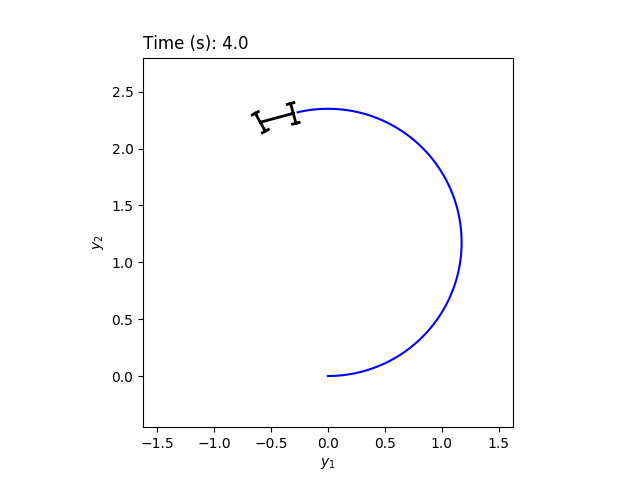
\includegraphics[width=0.7\textwidth]{img/animation}
	\caption{Car animation}
	\label{fig:animation}
\end{figure}
\end{document}
